%%%%%%%%%%%%%%%%%%%%%%%%%%%%%%%%%%%%%%%%%%%%%%%%%%

%% Tufte Working Papers (ISSN 2735-6043)
%% Bastián González-Bustamante (ed.)
%% https://training-datalab.com/tufte-working-papers/
%% https://github.com/training-datalab/tufte-working-papers/blob/master/LICENSE-CC.md
%% https://github.com/training-datalab/tufte-working-papers/blob/master/LICENSE-LPPL.md

%%%%%%%%%%%%%%%%%%%%%%%%%%%%%%%%%%%%%%%%%%%%%%%%%%

\documentclass[a4paper]{tufte-handout}
\usepackage{marvosym}
\usepackage[spanish]{babel}

%%%%%%%%%%%%%%%%%%%%%%%%%%%%%%%%%%%%%%%%%%%%%%%%%%

\title{Aplicación de ForceAtlas2, un algoritmo de diseño gráfico continuo, para el estudio de las élites \thanks{Este trabajo es una versión revisada de la ponencia presentada en el simposio ``\'Elites pol\'itico-administrativas: Delineando una agenda de investigaci\'on'' organizado en la Universidad de Santiago de Chile en noviembre de 2018.}
\\~\\~\\} 

\author{{\normalfont Basti\'an Gonz\'alez-Bustamante} \thanks{PRS DPhil (PhD) in Politics, Department of Politics and International Relations {\itshape \&} St Hilda's College, University of Oxford. Profesor Instructor, Departamento de Gesti\'on y Pol\'iticas P\'ublicas, Facultad de Administraci\'on y Econom\'ia, Universidad de Santiago de Chile (USACH). ORCID iD: \href{https://orcid.org/0000-0003-1510-6820}{\textcolor{blue}{0000-0003-1510-6820}}}}
\date{{\normalfont \normalsize \vspace{-1mm}University of Oxford} \\ {\normalfont \normalsize Universidad de Santiago de Chile} \\ {\LARGE \Letter} \href{mailto:bastian.gonzalezbustamante@politics.ox.ac.uk}{\textcolor{blue}{\normalfont \normalsize bastian.gonzalezbustamante@politics.ox.ac.uk}} \\~\\
{\normalfont Carla Cisternas} \thanks{Asistente de Investigaci\'on, Departamento de Gesti\'on y Pol\'iticas P\'ublicas, Facultad de Administraci\'on y Econom\'ia, Universidad de Santiago de Chile (USACH). ORCID iD: \href{https://orcid.org/0000-0001-7948-6194}{\textcolor{blue}{0000-0001-7948-6194}}} \\ {\normalfont \normalsize Universidad de Santiago de Chile} \\ 
{\LARGE \Letter} \href{mailto:carla.cisternas@usach.cl}{\textcolor{blue}{\normalfont \normalsize carla.cisternas@usach.cl}}
} 

%%%%%%%%%%%%%%%%%%%%%%%%%%%%%%%%%%%%%%%%%%%%%%%%%%

\hyphenation{Latino-america-na Elecci\'on eleccio-nes}

%%%%%%%%%%%%%%%%%%%%%%%%%%%%%%%%%%%%%%%%%%%%%%%%%%

\usepackage{graphicx} 
  \setkeys{Gin}{width=\linewidth,totalheight=\textheight,keepaspectratio}
  \graphicspath{{graphics/}} 
\usepackage{amsmath}  
\usepackage{booktabs} 
\usepackage{units}    
\usepackage{multicol} 
\usepackage{lipsum}   
\usepackage{fancyvrb} 
  \fvset{fontsize=\normalsize}

\newcommand{\doccmd}[1]{\texttt{\textbackslash#1}}
\newcommand{\docopt}[1]{\ensuremath{\langle}\textrm{\textit{#1}}\ensuremath{\rangle}}
\newcommand{\docarg}[1]{\textrm{\textit{#1}}}
\newcommand{\docenv}[1]{\textsf{#1}}
\newcommand{\docpkg}[1]{\texttt{#1}}
\newcommand{\doccls}[1]{\texttt{#1}}
\newcommand{\docclsopt}[1]{\texttt{#1}}
\newenvironment{docspec}{\begin{quote}\noindent}{\end{quote}}

%%%%%%%%%%%%%%%%%%%%%%%%%%%%%%%%%%%%%%%%%%%%%%%%%%

 \pdfinfo{
   /Author (Basti\'an Gonz\'alez-Bustamante)
   /Title  (Aplicación de ForceAtlas2, un algoritmo de diseño gráfico continuo, para el estudio de las élites)
   Subject (Tufte Working Papers)
}

%%%%%%%%%%%%%%%%%%%%%%%%%%%%%%%%%%%%%%%%%%%%%%%%%%

\addto\captionsspanish{
\def\tablename{Tabla}
\def\figurename{Figura}
}

\usepackage{subfig}
\usepackage{emerald}
\usepackage[T1]{fontenc}
\usepackage{multirow} 
\usepackage{hyperref}
\usepackage{xcolor, colortbl}

%%%%%%%%%%%%%%%%%%%%%%%%%%%%%%%%%%%%%%%%%%%%%%%%%%

\usepackage[final]{pdfpages}

\usepackage{fontawesome}

\begin{document}


\includepdf[pages=1]{../../covers/cover-001/cover-issue-001.pdf}

\includepdf[pages=2]{../../covers/cover-001/cover-issue-001.pdf}

\maketitle

\vspace{8mm}
\justify{\small {\bfseries Resumen:} Este documento de trabajo prueba un algoritmo alternativo para los períodos legislativos analizados por González-Bustamante y Cisternas (2016) en Chile entre 1990 y 2014. Se utiliza específicamente ForceAtlas2, el cual es un algoritmo de diseño gráfico continuo desarrollado por Jacomy et al. (2014) basado en un diseño dirigido por fuerza. Se analiza\marginnote{{\itshape {\bfseries Palabras clave:} \'Elites; capital político, carreras legislativas; Análisis de Redes Sociales; Chile.}} la composición social, militancia y los antecedentes educativos para identificar el nivel de homogeneidad en cada legislatura.}\\~\\

{\noindent \LARGE \itshape Applying ForceAtlas2, a Continuous Graph Layout Algorithm, to the Elites Study}\\

\justify{\small {\bfseries Abstract:} This working paper tests an alternative algorithm for the legislative periods analysed by González-Bustamante and Cisternas (2016) in Chile between 1990 and 2014. Specifically, ForceAtlas2 is used, which is a continuous graph layout algorithm developed by Jacomy et al. (2014) based on a force-directed design.\marginnote{{\itshape {\bfseries Keywords:} Elites; political capital, legislative careers; Social Network Analysis; Chile.}} The social composition, partisanship and educational background are analysed in order to identify the level of homogeneity in each legislature.}

%%%%%%%%%%%%%%%%%%%%%%%%%%%%%%%%%%%%%%%%%%%%%%%%%%

~\vfill
{\noindent \bfseries Nro. 1 | 2020}\\
{\noindent González-Bustamante, B., {\itshape \&} Cisternas, C. (2020). Aplicación de ForceAtlas2, un algoritmo de diseño gráfico continuo, para el estudio de las élites. {\itshape Tufte Working Papers}, 1, 1-15. {\scshape doi:} \href{https://doi.org/10.31235/osf.io/gxrkc}{\textcolor{blue}{10.31235/osf.io/gxrkc}}}\pagebreak

%%%%%%%%%%%%%%%%%%%%%%%%%%%%%%%%%%%%%%%%%%%%%%%%%%

%% \vspace{8mm}
\section[Introducci\'on] {{\normalfont Introducci\'on} \footnote{Esta investigaci\'on fue parcialmente financiada por los proyectos ANID/FONDECYT/1130054 y USA1498.37 de la Universidad de Santiago de Chile. Los autores declaran no tener potenciales conflictos de interés con respecto a esta investigación.}}

%%%%%%%%%%%%%%%%%%%%%%%%%%%%%%%%%%%%%%%%%%%%%%%%%%

\justify{En Gonz\'alez-Bustamante y Cisternas (2016) se analiz\'o la composici\'on social de las \'elites pol\'iticas en el poder legislativo chileno, espec\'ificamente en la C\'amara de Diputados durante el per\'iodo 1990-2014. En aquel art\'iculo se abordaron las caracter\'isticas personales y las tasas de reelecci\'on de todos los diputados que ejercieron durante aquellos a\~nos ({\itshape n} = 720). Adem\'as, con indicadores simples, an\'alisis de cl\'uster y An\'alisis de Redes Sociales ({\itshape Social Network Analysis}, SNA), se midi\'o el grado de homogeneidad y el trasfondo educacional de las seis legislaturas del per\'iodo. Los hallazgos evidenciaron que la composici\'on social de las legislaturas fue m\'as homog\'enea y, por tanto, existieron redes m\'as densas, mientras m\'as antigua fuese la legislatura. En otras palabras, mientras m\'as cerca de la transici\'on democr\'atica de fines de la d\'ecada de 1980, mayor homogeneidad social tenían las legislaturas\footnote{Para una reflexi\'on te\'orica sobre \'elites pol\'iticas y poder legislativo v\'ease el art\'iculo original.}.}

\justify{En t\'erminos metodol\'ogicos se utiliz\'o {\itshape Hirschman-Herfindahl index} (HHI), tradicionalmente usado para medir concentraciones de mercado, con el objetivo de evaluar la homogeneidad del trasfondo educacional en las distintas legislaturas\footnote{Joignant (2014) utiliz\'o el HHI para evaluar la concentraci\'on de la parentela pol\'itica en las elecciones de 2013.}. Esto se complement\'o con an\'alisis de cl\'uster con un algoritmo {\itshape K-means clustering} o de agrupamiento no jer\'arquico, en l\'inea con los an\'alisis de Gonz\'alez-Bustamante y Olivares (2015) sobre subsecretarios chilenos entre 1990 y 2014. Se trabaj\'o espec\'ificamente con {\itshape Caliński-Harabasz index} con m\'etodo Hellinger para determinar el n\'umero de cl\'usteres. Para esto se utilizaron caracter\'isticas individuales de los diputados como sexo, militancia y variables relacionadas con su trasfondo educacional.}

\justify{Aquellas variables tambi\'en se utilizaron para un SNA, el cual permite identificar interrelaciones y v\'inculos en un grupo determinado (Friedkin, 1981; Hanneman y Riddle, 2005; Wasserman y Faust, 1994). Se utiliz\'o el algoritmo Fruchterman y Reingold (1991), una modificaci\'on del modelo {\itshape spring-embedder} de Eades (1984), donde se asimila el grafo a un sistema de part\'iculas de masa en el cual los {\itshape nodos} son las part\'iculas y los {\itshape edges} o v\'inculos operan como resortes de repulsi\'on\footnote{La met\'afora cl\'asica de Eades (1984) indicaba que para dise\~nar un gr\'afico se deb\'ia reemplazar los v\'ertices ({\itshape nodos}) por anillos de acero y los v\'inculos ({\itshape edges}) por un resorte para formar un sistema mec\'anico. Los v\'ertices se colocan en un dise\~no inicial que se deja en libertad para que las fuerzas de los anillos muevan al sistema a un nuevo estado m\'inimo de energ\'ia.}.}

\justify{Efectivamente, el SNA permite observar vínculos y medir interrelaciones en un grupo (Cisternas y Vásquez, 2018; González-Bustamante y Cisternas, 2016). En este sentido, es una técnica con diversas aplicaciones en el campo de la sociología y, en menor medida, en la ciencia política. También se utiliza bastante en análisis bibliométricos para evaluar la relación entre estructuras sociales, referenciación y coautorías (Cronin y Shaw, 2002; Cisternas y González-Bustamante, 2016; White, 2001).}

\justify{En este contexto, tal como se indica en González-Bustamante (2020) y Olivares et al. (2020), si bien el SNA aplicado al estudio de las \'elites pol\'iticas tiene diversas potencialidades, pueden existir algunos problemas cuando se basa en la idea de que los atributos se cristalizan en perspectivas ideol\'ogicas u ontol\'ogicas. Esto porque el concepto de cristalizaci\'on se asocia, por ejemplo, al {\itshape habitus} de Bourdieu (1980), por tanto, opera una estructura estructurante que se transforma en redes de cooperaci\'on. Sin embargo, puede ser que el v\'inculo no exista o que la relaci\'on sea conflictiva. Por otra parte, cuando se trabaja desde una perspectiva relacional, pueden existir problemas de deseabilidad social.}

\justify{Este documento de trabajo eval\'ua un algoritmo alternativo para las legislaturas analizadas por Gonz\'alez-Bustamante y Cisternas (2016). Espec\'ificamente se utiliza ForceAtlas2, un algoritmo de dise\~no gr\'afico continuo desarrollado por Jacomy et al. (2014) con base en un dise\~no dirigido por fuerza ({\itshape force-directed}). Si bien el algoritmo Fruchterman y Reingold (1991) tambi\'en es dirigido por fuerza, los modelos de energ\'ia var\'ian ya que cada algoritmo se basa en f\'ormulas diferentes para la fuerza de atracci\'on y de repulsi\'on.}

\justify{El objetivo principal de este trabajo es demostrar que introduciendo mejoras, como el uso del algoritmo ForceAtlas2 y ajustes específicos en su configuración, es posible realizar un análisis más detallados de las conexiones y la conformación de conglomerados en un grupo, en este caso la élite legislativa chilena. Esto permite una evaluación visual más intuitiva de los niveles de homogeneidad y cierre social. Para cumplir con este objetivo, este documento se estructura en tres apartados. Primero, un apartado metodol\'ogico que detalla los datos y algoritmos usados. Segundo, los principales resultados de la aplicaci\'on de ForceAtlas2. Finalmente, un breve resumen de los principales hallazgos, l\'ineas futuras de investigaci\'on y límites.}

%%%%%%%%%%%%%%%%%%%%%%%%%%%%%%%%%%%%%%%%%%%%%%%%%%

\section[M\'etodo] {{\normalfont M\'etodo}}

%%%%%%%%%%%%%%%%%%%%%%%%%%%%%%%%%%%%%%%%%%%%%%%%%%

\subsection[Datos] {Datos}

\justify{De la misma forma que Gonz\'alez-Bustamante y Cisternas (2016), se utiliza una base de datos con informaci\'on electoral y biogr\'afica de los candidatos que compitieron en las elecciones de diputados en Chile entre 1989 y 2009 ({\itshape N} = 2.441). La base se elabora a partir de datos de Joignant (2014), Gonz\'alez-Bustamante (2014) e informaci\'on del Servicio Electoral de Chile (SERVEL)\footnote{Para informaci\'on detallada sobre bases de datos similares y trabajo emp\'irico reciente sobre \'elites en Chile v\'ease Gonz\'alez-Bustamante y Olivares (2018) y Maillet, Gonz\'alez-Bustamante y Olivares (2016).}. }

\begin{table}[h]
  \centering
  \fontfamily{ppl}\selectfont
   \smallskip\noindent\small Tabla 1 \\ Candidaturas, electividad y reelecci\'on C\'amara de Diputados en Chile (1990-2014) \\~\\
  \begin{tabular}{c c c c c}
    \toprule
    Elecci\'on & Legislatura & Candidatos & Electividad & Reelecci\'on \\
    \midrule
    1989 & 1990-1994 & 419 & 28,6 & -- \\
    1993 & 1994-1998 & 384 & 31,3 & 58,3 \\
    1997 & 1998-2002 & 442 & 27,2 & 60,8 \\
    2001 & 2002-2006 & 381 & 31,5 & 61,7 \\
    2005 & 2006-2010 & 386 & 31,1 & 64,2 \\
    2009 & 2010-2014 & 429 & 28,0 & 61,7 \\
    \midrule
     & & 2.441 & 29,5 & 61,3 \\
    \bottomrule
  \end{tabular}
  \\~\\ \smallskip\noindent\scriptsize Fuente: Adaptaci\'on de Gonz\'alez-Bustamante y Cisternas (2016) con datos de Joignant (2014), Gonz\'alez-Bustamante (2014) y del Servicio Electoral de Chile.
\end{table}

\justify{El an\'alisis se realiza sobre los diputados electos ({\itshape n} = 720), que corresponden a 329 individuos debido a las altas tasas de incumbencia y reelecci\'on en la C\'amara de Diputados chilena (Tabla 1)\footnote{Tal como indican Gonz\'alez-Bustamante y Cisternas (2016) estos datos difieren levemente de los de Bunker y Navia (2015), pues se reporta un diputado menos reelecto en 2001, lo que fue verificado con informaci\'on actualizada del Servicio Electoral. Hay otras cifras de reelecci\'on, como las de Salda\~na (2014), que no concuerdan con estos datos ni con los de Bunker y Navia.}. Los datos de reelecci\'on que se presentan corresponden a los incumbentes que tuvieron \'exito en su mismo distrito. El promedio se eleva a 62,8\% si se considera a aquellos que, estrat\'egicamente, buscaron su reelecci\'on en otro distrito.}

\subsection[Algoritmos] {Algoritmos}

\justify{El modelo {\itshape spring-embedder} de Eades (1984) opera con una f\'ormula de atracci\'on $F_{\alpha} = -k * d$, donde $d$ es una distancia geom\'etrica entre dos {\itshape nodos} y $k$ un ajuste para el escalamiento de la red, y una f\'ormula de repulsi\'on como si se tratase de part\'iculas el\'ectricamente cargadas $F_{r} = k /d^{2}$. La f\'ormula cl\'asica de Fruchterman y Reingold (1991), utilizada por Gonz\'alez-Bustamante y Cisternas (2016), constituye una modificaci\'on basada en f\'ormulas de atracci\'on $F_{\alpha} = d^{2} / k$ y repulsi\'on $F_{r} = -k^{2} / d$.}

\justify{En general, la diferencia m\'as relevante entre los algoritmos dirigidos por fuerza es el rol de la distancia en la espacializaci\'on del gr\'afico (Noack, 2007a; v\'ease tambi\'en Jacomy et al., 2014). La fuerza depende de la distancia entre los {\itshape nodos} y la relaci\'on entre ambas puede ser lineal, exponencial o logar\'itmica (Jacomy et al., 2014).  En el modelo cl\'asico de Eades (1984) la relaci\'on es lineal. Por tanto, la ecuaci\'on de un modelo atracci\'on por fuerza lineal sin constante ser\'ia (1).}

\begin{equation} 
F_{\alpha}(n_{1}, n_{2}) = d(n_{1}, n_{2})
\end{equation}

\justify{Si se utiliza el concepto de modelo de energ\'ia o de atracci\'on-repulsi\'on de Noack (2009), se puede especificar una notaci\'on simple para cada algoritmo basada en el exponente de la distancia de las f\'ormulas de $F_{\alpha}$ y $F_{r}$. Entonces, para {\itshape spring-embedder} ser\'ia (1, -2), Fruchterman y Reingold (2, -1), y ForceAtlas (1, -1). Para ForceAtlas2 la f\'ormula de repulsi\'on toma en cuenta el grado de los {\itshape nodos} ({\itshape deg}) con base en un recuento de los {\itshape edges} conectados, siendo muy similar a la f\'ormula de Noack (2007a) con un ajuste de +1 para asegurar que $deg = 0$ tenga algo de fuerza de repulsi\'on (2) (Jacomy et al., 2014). En este trabajo se utiliza $k_{r} = 1,5$.

\begin{equation} 
F_{r}(n_{1}, n_{2}) = k_{r}\frac{(deg(n_{1}) + 1) (deg(n_{2}) + 1)}{d(n_{1}, n_{2})}
\end{equation}

\justify{Por otra parte, se utiliza un modelo logar\'itmico de fuerza basado en el modelo de energ\'ia LinLog de Noack (2007b), con un ajuste similar al de la f\'ormula de repulsi\'on (3) (Jacomy et al., 2014).}

\begin{equation} 
F_{\alpha}(n_{1}, n_{2}) = log (1 + d(n_{1}, n_{2}))
\end{equation}

\justify{Adem\'as, se utiliza un efecto de gravedad $F_{g}(n)$ para prevenir la desconexi\'on de componentes que formen islas alejadas en el grafo (4). En este trabajo se utiliza $k_{g} = 1,5$.}

\begin{equation} 
F_{g} = k_{g} (deg(n) + 1)
\end{equation}

\justify{Por \'ultimo, se utilizan dos efectos propios de ForceAtlas2: disuadir centros de actividad ({\itshape Hubs}) y evitar solapamiento (Jacomy et al., 2014). El efecto de disuadir {\itshape Hubs} permite que {\itshape nodos} con mayor cantidad de v\'inculos dirigidos hac\'ia si mismos ocupen posiciones centrales. Para esto se divide la fuerza de atracci\'on de cada {\itshape nodo} por su grado m\'as uno (5).}

\begin{equation} 
F_{\alpha}(n_{1}, n_{2}) = \frac{d(n_{1}, n_{2})}{deg(n_{1} + 1)}
\end{equation}

\justify{El efecto para evitar solapamiento, por otra parte, mejora la visualizaci\'on considerando el tama\~no de los {\itshape nodos} y su distancia $d^{`} (n_{1}, n_{2}) = d (n_{1}, n_{2}) - size(n_{1}) - size(n_{2})$. Si $d^{`} (n_{1}, n_{2}) > 0$ no hay solapamiento, por lo cual se utiliza la ecuaci\'on de repulsi\'on normal. Sin embargo, si $d^{`} (n_{1}, n_{2}) < 0$, entonces $F_{\alpha} (n_{1}, n_{2}) = 0$ y la repulsi\'on ser\'a m\'as fuerte (6) (Jacomy et al., 2014).}

\begin{equation} 
F_{r}(n_{1}, n_{2}) = k^{`}_{r}(deg(n_{1}) + 1)(deg(n_{2}) + 1)
\end{equation}

\justify{Adem\'as, siguiendo a Blondel et al. (2008), se utiliza un algoritmo de modularidad donde cada {\itshape nodo} $i$ se sit\'ua con sus {\itshape alters} $j$ y se eval\'ua la ganancia de modularidad al eliminar $i$. El {\itshape nodo} entonces se coloca en la comunidad $C$ donde la ganancia es m\'axima siempre que sea positiva, si es negativa se mantiene en la posici\'on inicial. Este proceso se itera hasta que no existen movimientos que puedan mejorar el nivel de modularidad (Newman y Girvan, 2004).  La modularidad $\Delta Q$ se calcula considerando los v\'inculos $in$ dentro de $C$, los v\'inculos $tot$ hacia {\itshape nodos} dentro de $C$, la suma $k_{i}$ de enlaces hacia el {\itshape nodo} $i$ cuyo aporte se eval\'ua, y la suma de todos los v\'inculos de la red $m$ (7) (Blondel et al., 2008)\footnote{Tambi\'en se calcula el di\'ametro de la red con el algoritmo de centralidad de intermediaci\'on de Brandes (2001). Esto permite estimar el sendero m\'as extenso entre cualquier {\itshape nodo} de la red.}.}

\begin{equation} 
\Delta Q = \left[\frac{\sum_{in} + 2k_{i, in}}{2m} - \left(\frac{\sum_{tot} + k_{i}}{2m}\right)^{2}\right] - \left[\frac{\sum_{in}}{2m} - \left(\frac{\sum_{tot}}{2m}\right)^{2} - \left(\frac{k_{i}}{2m}\right)^{2}\right]
\end{equation}

%%%%%%%%%%%%%%%%%%%%%%%%%%%%%%%%%%%%%%%%%%%%%%%%%%

\section[Resultados] {{\normalfont Resultados}}

%%%%%%%%%%%%%%%%%%%%%%%%%%%%%%%%%%%%%%%%%%%%%%%%%%

\subsection[Fuchterman y Reingold vs. ForceAtlas2] {Fuchterman y Reingold vs. ForceAtlas2}

\justify{A continuaci\'on, se presentan los grafos por cada legislatura. Aquellos graficados con el algoritmo Fruchterman y Reingold son los originales de Gonz\'alez-Bustamante y Cisternas (2016), pero con colores y {\itshape edges} curvos. Se utiliza una paleta de colores que distingue la militancia pol\'itica. Los grafos con el algoritmo ForceAtlas2 utilizan la misma paleta de colores y los valores de gravedad y repulsi\'on estipulados en el apartado metodol\'ogico.}

\begin{figure}[h!]
\captionsetup[subfigure]{labelformat=empty}
  \centering
  \smallskip\noindent\small Figura 1 \\ Legislatura 1990-1994
  \subfloat[Fruchterman y Reingold]{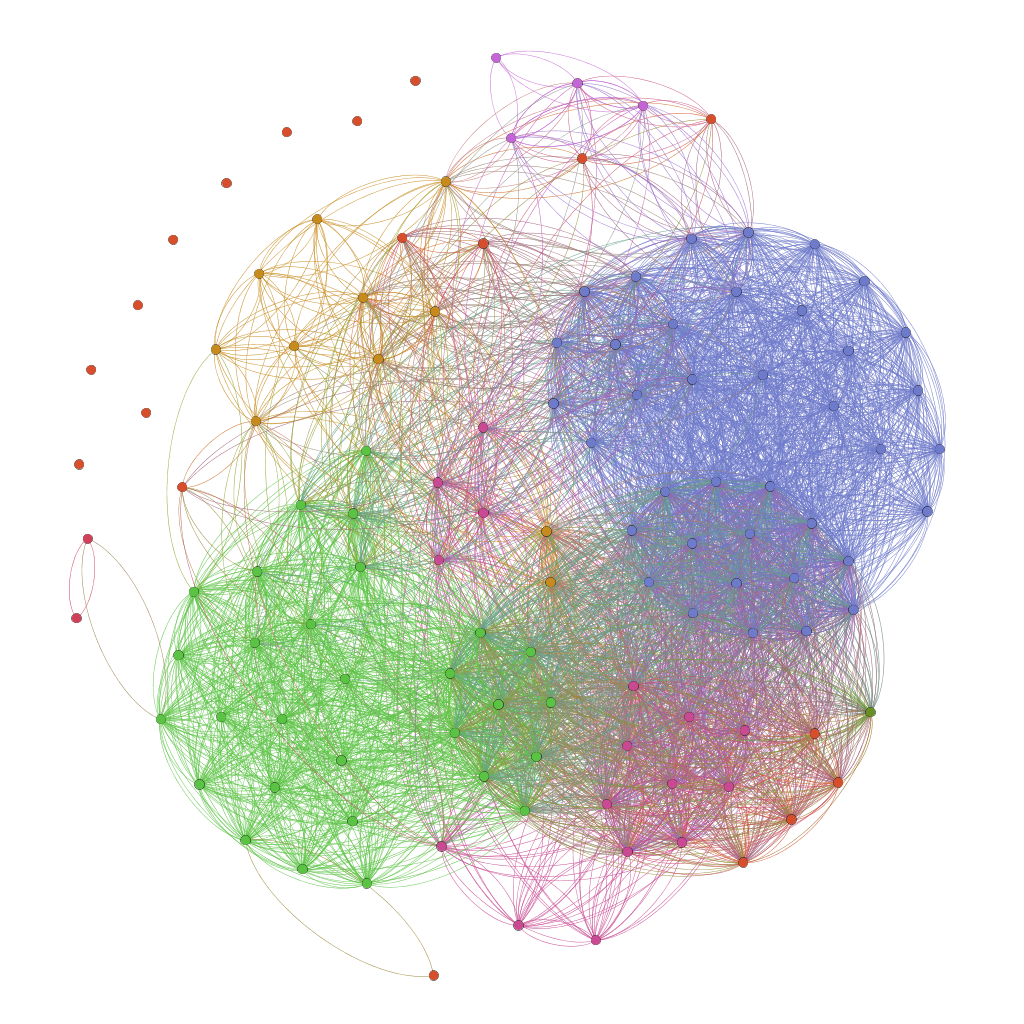
\includegraphics[width=.45\linewidth]{../01.Figures/FR-1990}}
  \subfloat[ForceAtlas2]{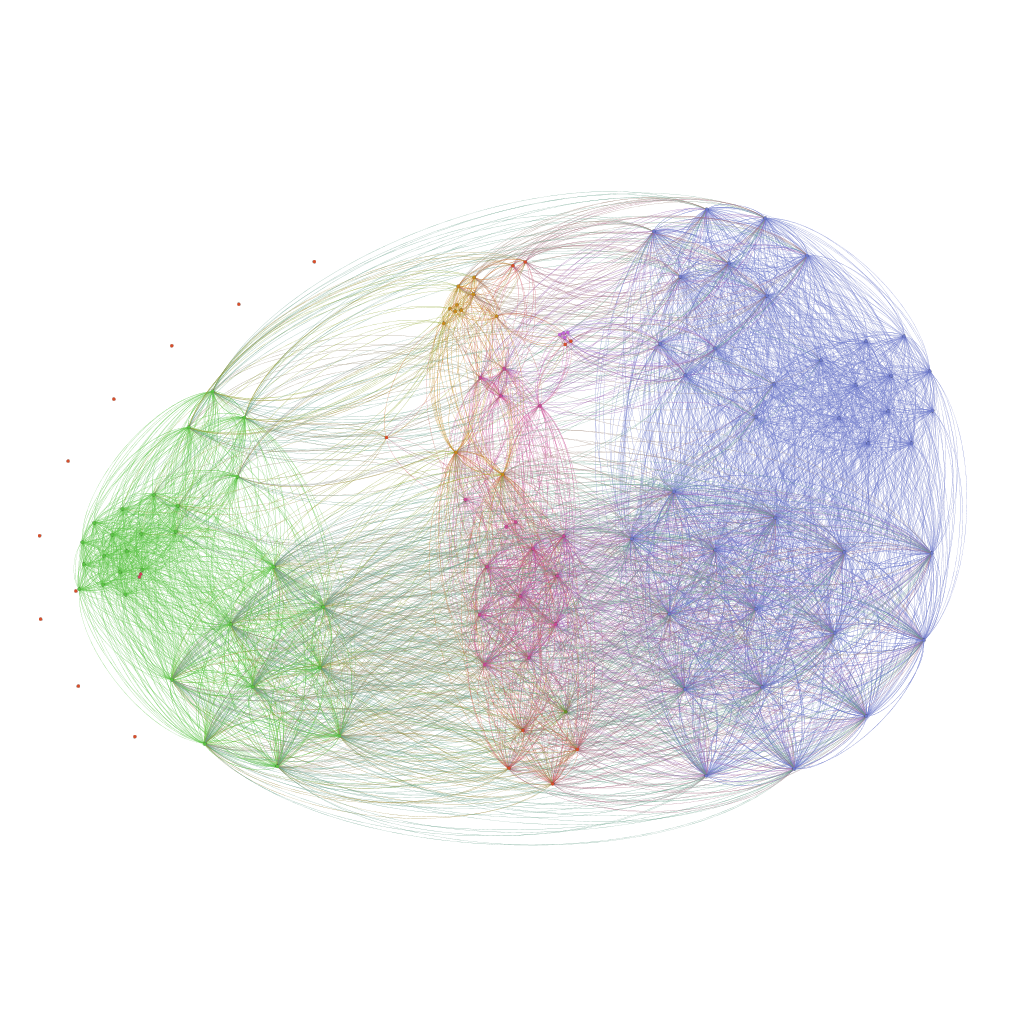
\includegraphics[width=.5\linewidth]{../01.Figures/FA2-1990}}
  \\ \smallskip\noindent\scriptsize Nota: El grafo original con el algoritmo Fruchterman y Reingold fue publicado en escala de grises. En esta versi\'on se utilizan colores para indicar militancia pol\'itica: PDC azul purp\'ureo, RN malaquita, IND tomate, PPD violeta, UDI anaranjado, PR malva, PAIS carmes\'i y PH verde oscuro.\\
  Fuente: Elaboraci\'on propia con datos de Gonz\'alez-Bustamante y Cisternas (2016).
\end{figure}

\justify{En la Figura 1 con ForceAtlas2 se aprecian con mayor claridad los dos grandes conglomerados de {\itshape nodos} compuestos por el Partido Dem\'ocrata Cristiano (PDC) y Renovaci\'on Nacional (RN). Con el algoritmo Fruchterman y Reingold se aprecia que un subgrupo de {\itshape nodos} de RN tiende a operar como intermediarios. En el grafo con ForceAtlas2 se aprecia de mejor forma como parte del conglomerado tiene mayores conexiones con otros, a diferencia de un grupo m\'as cerrado con conexiones m\'as fuertes. El valor del grafo medio es 38,567, es decir, en promedio un {\itshape nodo} posee esa cantidad de {\itshape alters} vecinos. El di\'ametro de la red es de cinco, es decir, esa es la m\'axima distancia que existe entre cualquier {\itshape nodo}. Por \'ultimo, la densidad de la red es de 0,324.}

\begin{figure}[h!]
\captionsetup[subfigure]{labelformat=empty}
  \centering
  \smallskip\noindent\small Figura 2 \\ Legislatura 1994-1998
  \subfloat[Fruchterman y Reingold]{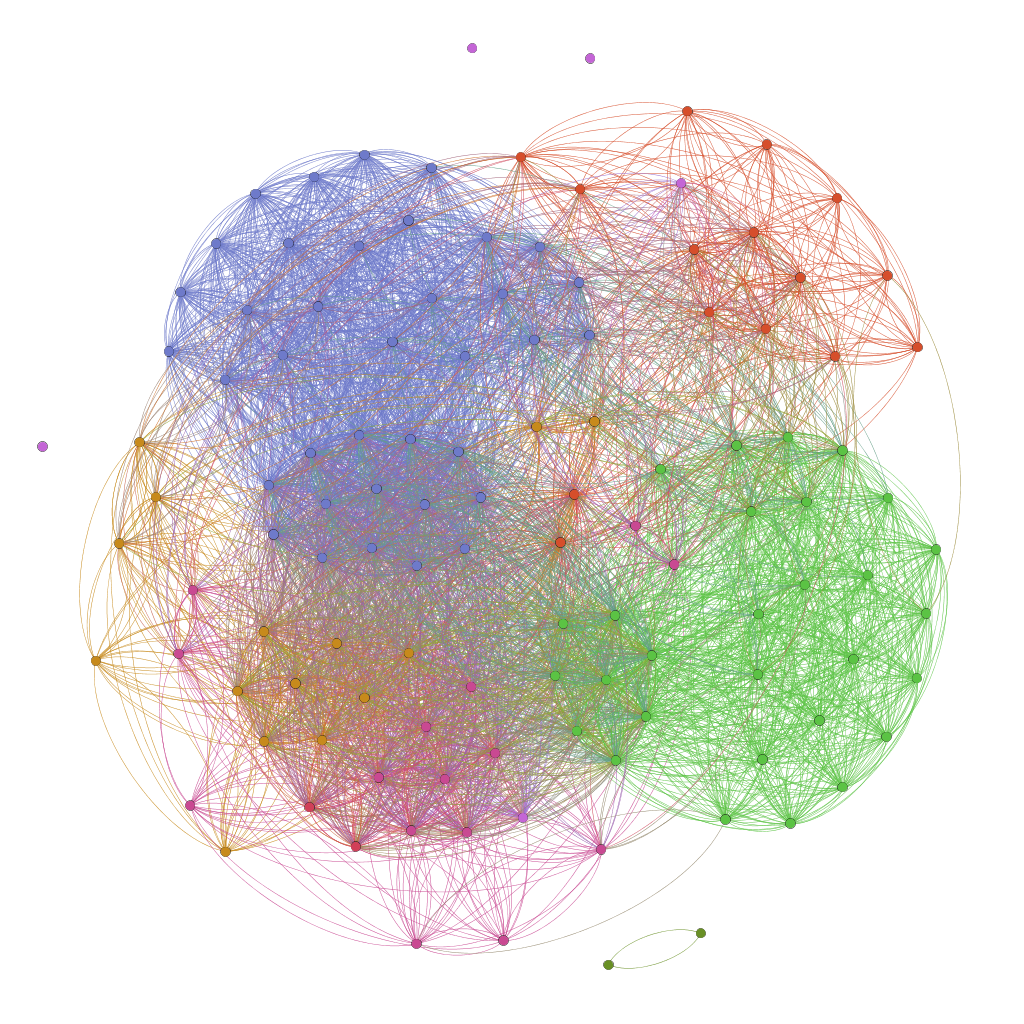
\includegraphics[width=.45\linewidth]{../01.Figures/FR-1994}}
  \subfloat[ForceAtlas2]{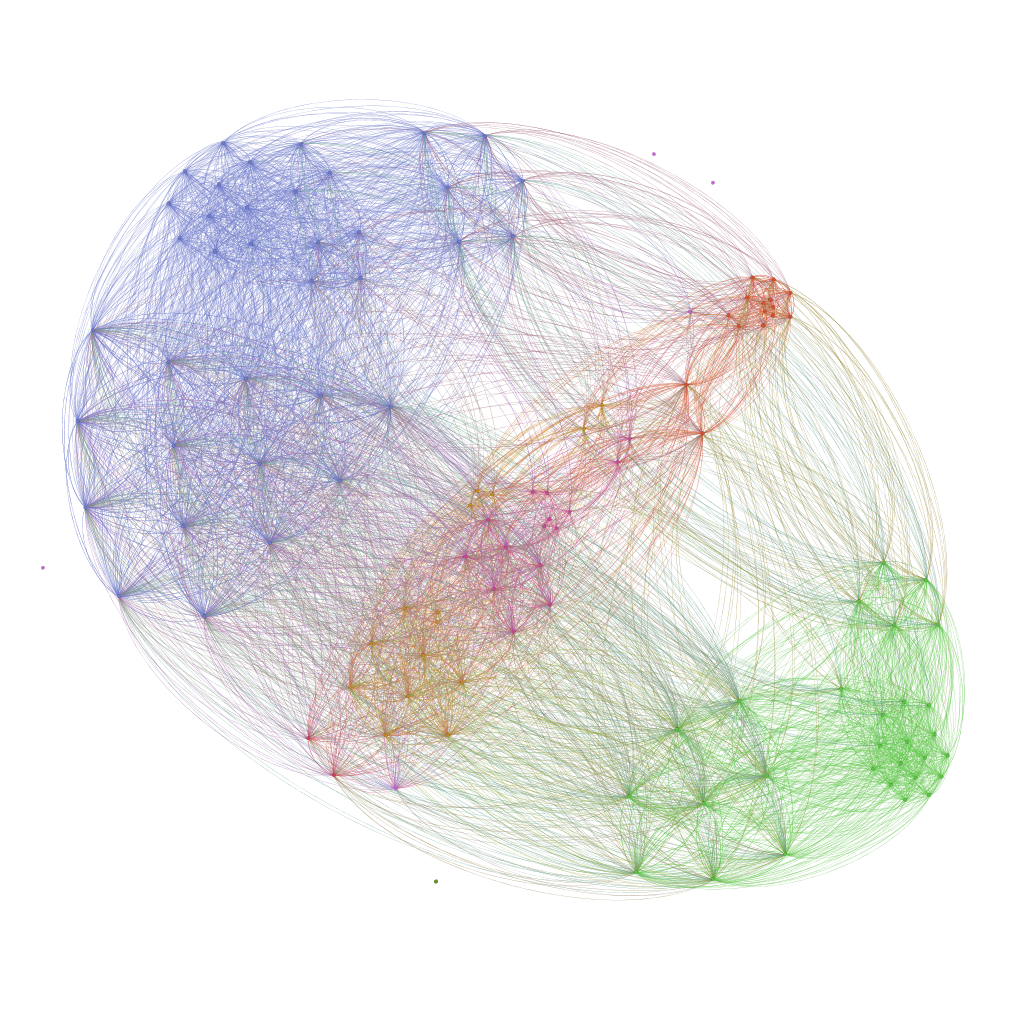
\includegraphics[width=.5\linewidth]{../01.Figures/FA2-1994}}
  \\ \smallskip\noindent\scriptsize Nota: El grafo original con el algoritmo Fruchterman y Reingold fue publicado en escala de grises. En esta versi\'on se utilizan colores para indicar militancia pol\'itica: PDC azul purp\'ureo, RN malaquita, UDI tomate, PS violeta, PPD anaranjado, IND malva, UCC carmes\'i y PR verde oscuro.\\
  Fuente: Elaboraci\'on propia con datos de Gonz\'alez-Bustamante y Cisternas (2016).
\end{figure}

\justify{La Figura 2 mantiene los patrones de la anterior, se aprecia un conglomerado de {\itshape nodos} del PDC que se alejan de del resto de la red, adem\'as de un conglomerado mixto entre el Partido Por la Democracia (PPD) y el Partido Socialista de Chile (PS). En este caso el algoritmo ForceAtlas2 tambi\'en permite una mejor visualizaci\'on. El grafo medio es de 42,667, el di\'ametro de tres y la densidad de 0,359. Si bien la densidad no var\'ia sustancialmente, es una red con menor di\'ametro que la anterior.}

\begin{figure}[h!]
\captionsetup[subfigure]{labelformat=empty}
  \centering
  \smallskip\noindent\small Figura 3 \\ Legislatura 1998-2002
  \subfloat[Fruchterman y Reingold]{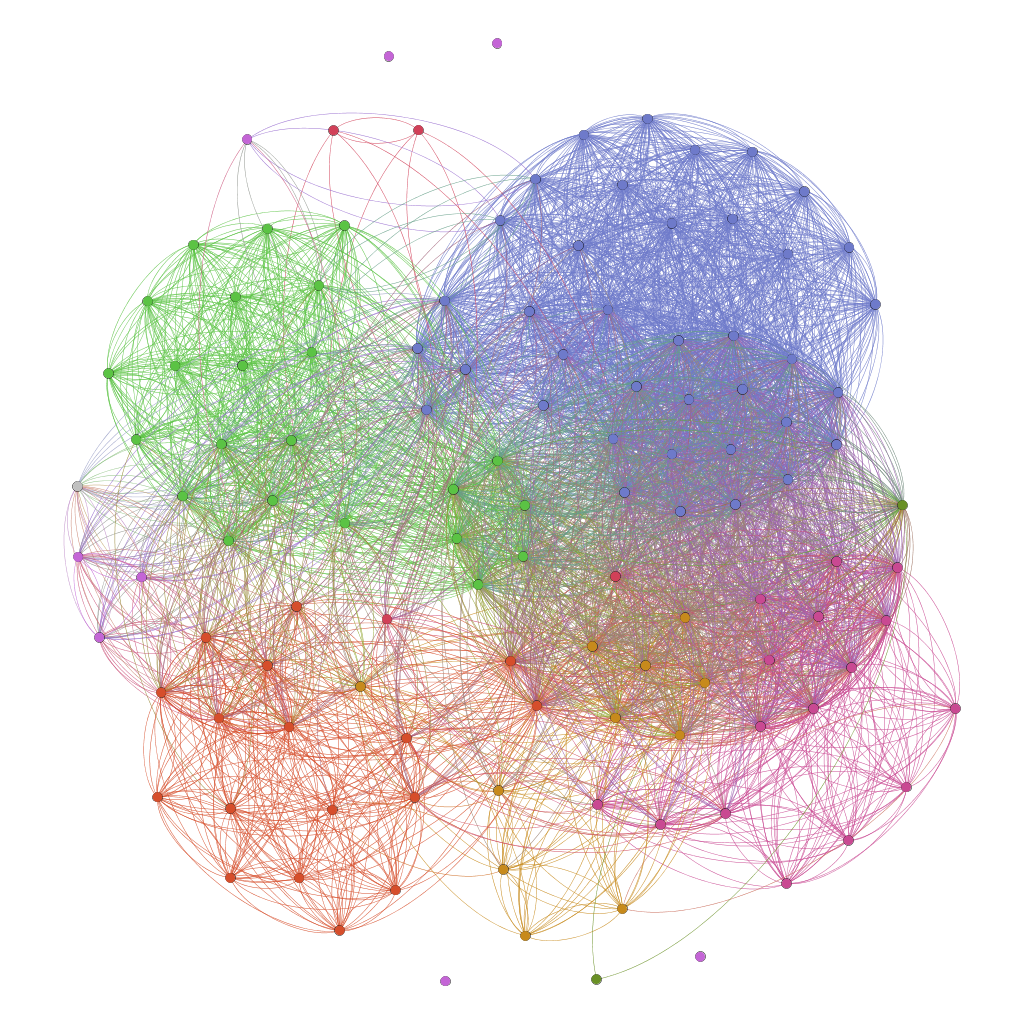
\includegraphics[width=.45\linewidth]{../01.Figures/FR-1998}}
  \subfloat[ForceAtlas2]{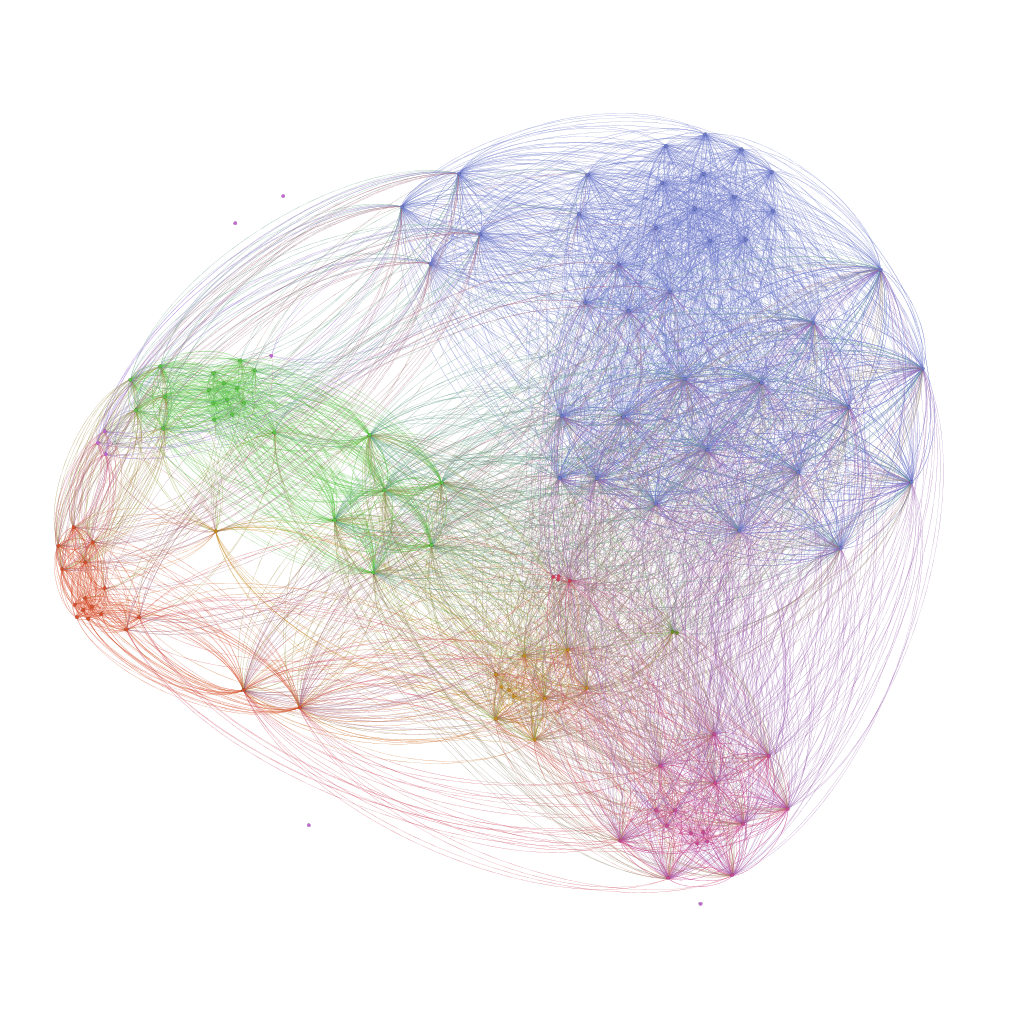
\includegraphics[width=.5\linewidth]{../01.Figures/FA2-1998}}
  \\ \smallskip\noindent\scriptsize Nota: El grafo original con el algoritmo Fruchterman y Reingold fue publicado en escala de grises. En esta versi\'on se utilizan colores para indicar militancia pol\'itica: PDC azul purp\'ureo, RN malaquita, UDI tomate, PPD violeta, PS anaranjado, IND malva, PRSD carmes\'i y UCCP verde oscuro.\\
  Fuente: Elaboraci\'on propia con datos de Gonz\'alez-Bustamante y Cisternas (2016).
\end{figure}

\justify{En la Figura 3 se puede apreciar un crecimiento de los {\itshape nodos} pertenecientes a la Uni\'on Dem\'ocrata Independiente (UDI), conglomerado que tiene lazos principalmente con RN, sus socios de coalici\'on. En el grafo con el algoritmo ForceAtlas2 se puede visualizar su constituci\'on de mejor forma: como un m\'odulo con fuertes conexiones entre s\'i y conexiones con RN, lo que los ubica en la periferia de la red. El grafo medio es de 39,183, el di\'ametro de la red cuatro y la densidad 0,329.}

\begin{figure}[h!]
\captionsetup[subfigure]{labelformat=empty}
  \centering
  \smallskip\noindent\small Figura 4 \\ Legislatura 2002-2006
  \subfloat[Fruchterman y Reingold]{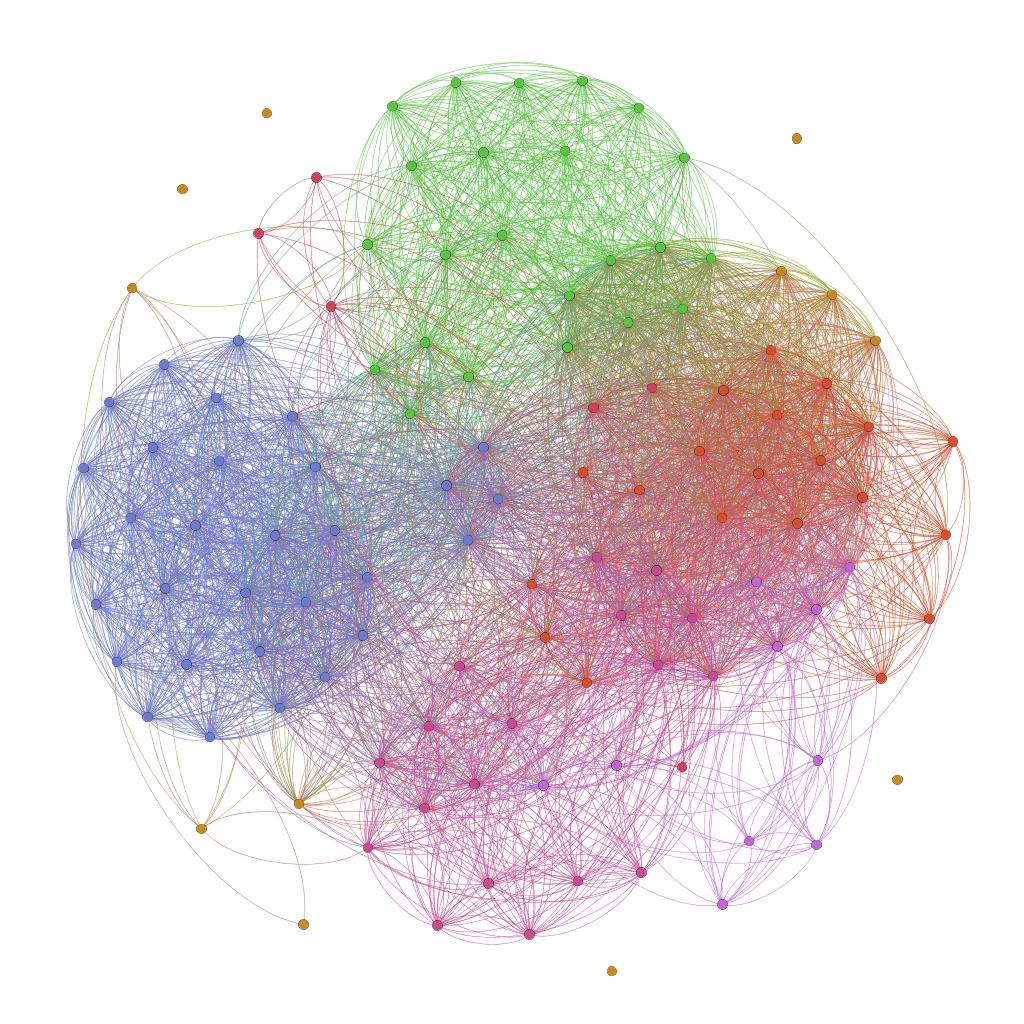
\includegraphics[width=.45\linewidth]{../01.Figures/FR-2002}}
  \subfloat[ForceAtlas2]{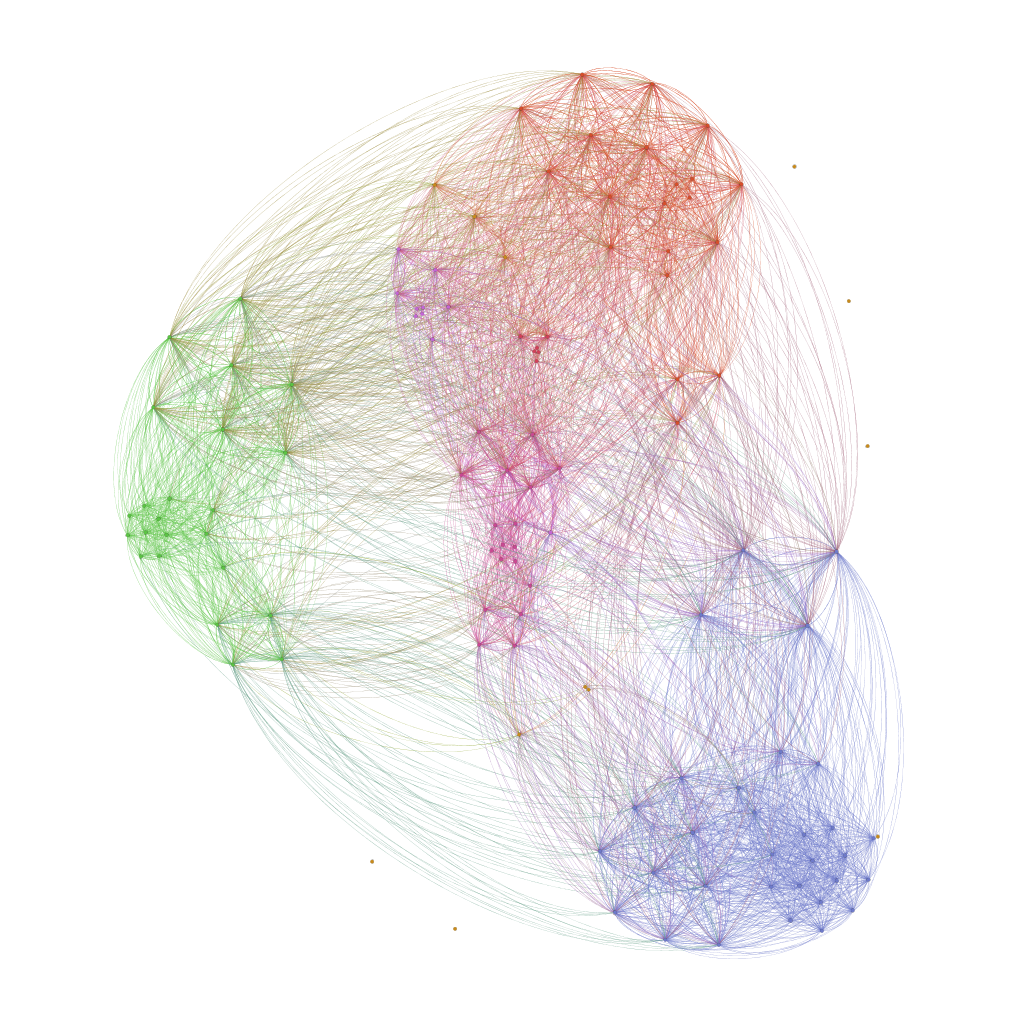
\includegraphics[width=.5\linewidth]{../01.Figures/FA2-2002}}
  \\ \smallskip\noindent\scriptsize Nota: El grafo original con el algoritmo Fruchterman y Reingold fue publicado en escala de grises. En esta versi\'on se utilizan colores para indicar militancia pol\'itica: UDI azul purp\'ureo, PDC malaquita, PPD tomate, RN violeta, IND anaranjado, PS malva y PRSD carmes\'i.\\
  Fuente: Elaboraci\'on propia con datos de Gonz\'alez-Bustamante y Cisternas (2016).
\end{figure}

\justify{En la Figura 4 se aprecia un crecimiento importante de la UDI. Aquello se percibe de mejor forma con la aplicaci\'on del algoritmo ForceAtlas2, como tambi\'en la posici\'on de intermediaci\'on que tienden a ocupar ciertos {\itshape nodos}. El grafo medio de la red es 34,767, el di\'ametro cuatro y la densidad 0,292.}

\begin{figure}[h!]
\captionsetup[subfigure]{labelformat=empty}
  \centering
  \smallskip\noindent\small Figura 5 \\ Legislatura 2006-2010
  \subfloat[Fruchterman y Reingold]{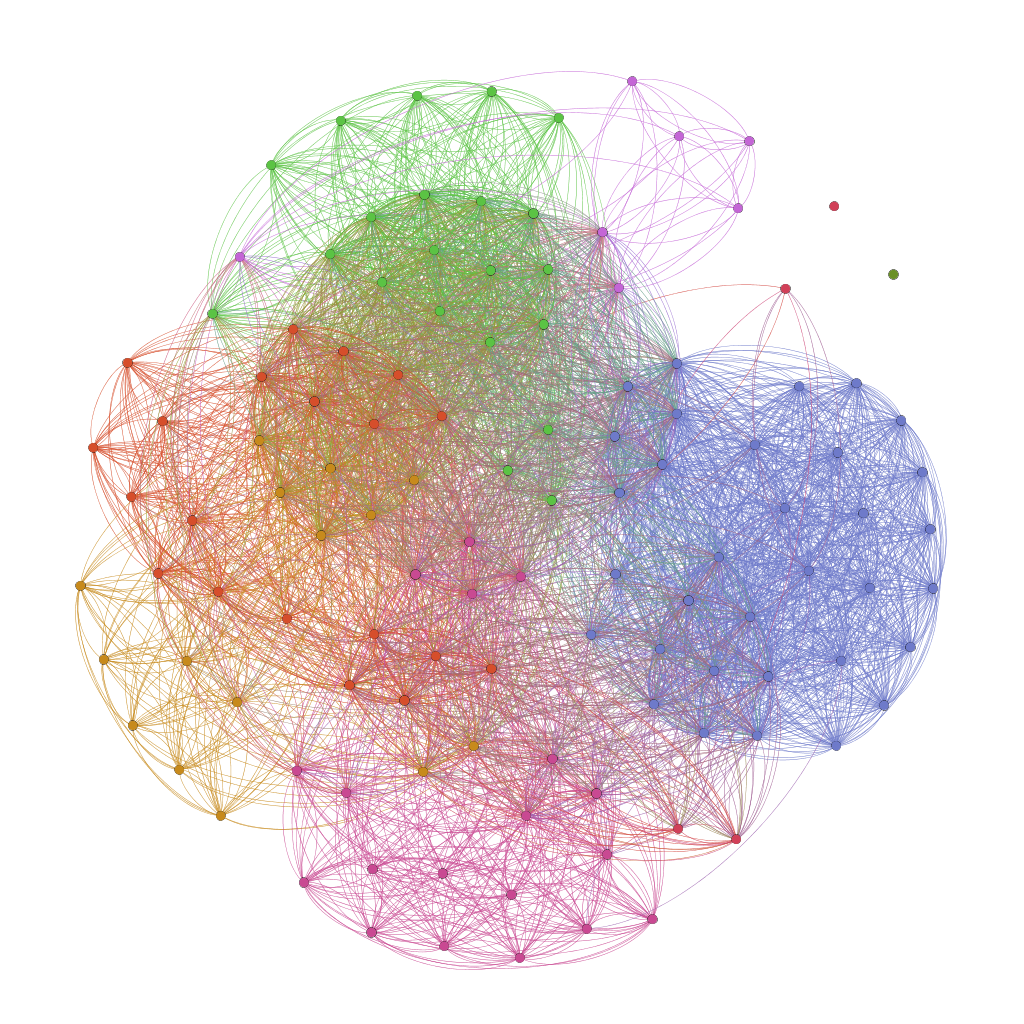
\includegraphics[width=.45\linewidth]{../01.Figures/FR-2006}}
  \subfloat[ForceAtlas2]{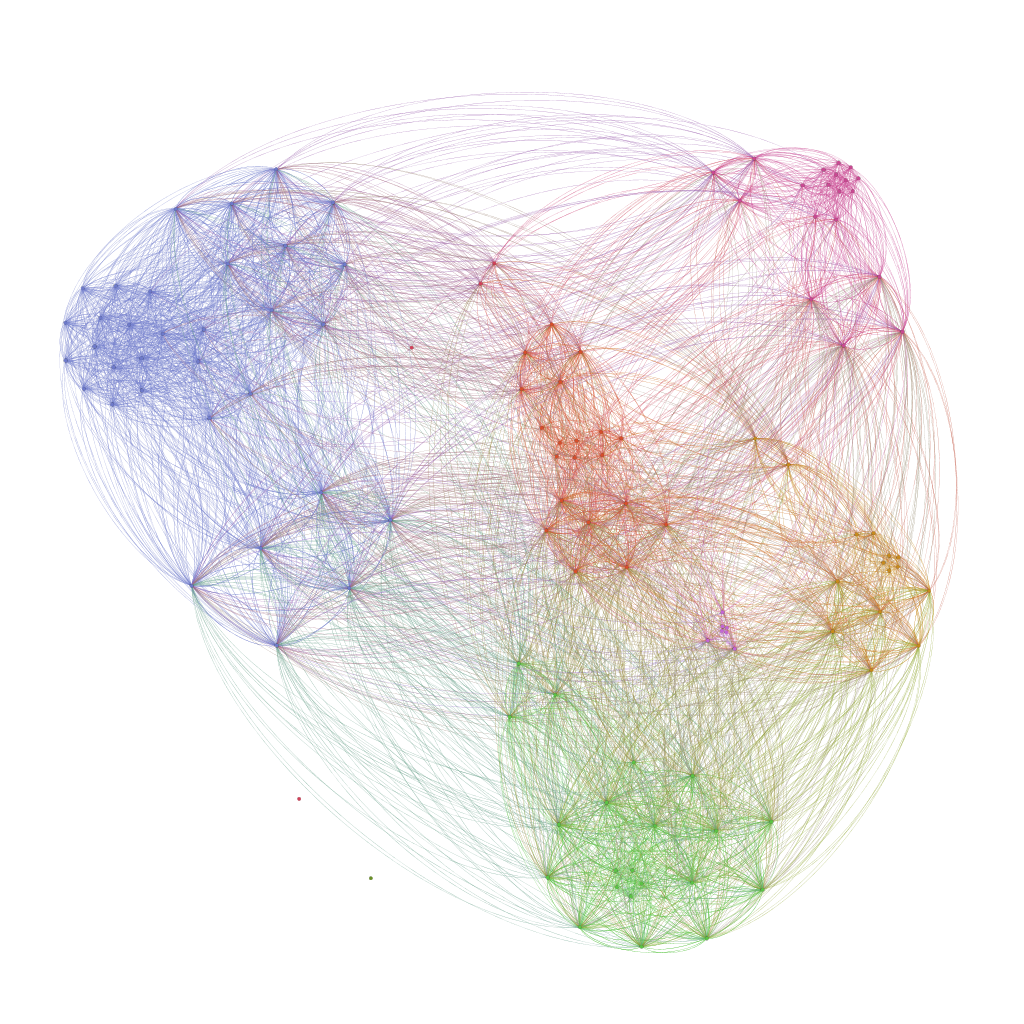
\includegraphics[width=.5\linewidth]{../01.Figures/FA2-2006}}
  \\ \smallskip\noindent\scriptsize Nota: El grafo original con el algoritmo Fruchterman y Reingold fue publicado en escala de grises. En esta versi\'on se utilizan colores para indicar militancia pol\'itica: UDI azul purp\'ureo, PPD malaquita, PDC tomate, RN violeta, PS anaranjado, PRSD malva, IND carmes\'i y PAR verde oscuro.\\
  Fuente: Elaboraci\'on propia con datos de Gonz\'alez-Bustamante y Cisternas (2016).
\end{figure}

\justify{En la Figura 5 tambi\'en se aprecian mejor las posiciones de intermediaci\'on en la red gracias al algoritmo ForceAtlas2. Es posible identificar mejor la cercan\'ia entre los conglomerados del PPD, PS y PDC. Adem\'as, mientras que con el algoritmo Fruchterman y Reingold RN no parece un conglomerado cohesionado, ForceAtlas2 permite apreciar dos grupos: uno fuertemente cohesionado en la periferia de la red y otro que opera como un intermediario entre los conglomerados de PPD, PS y PDC. El grafo medio de esta red es de 37,267, su di\'ametro cuatro y su densidad 0,313.}

\justify{Finalmente, en la Figura 6 se acent\'ua la preponderancia del cl\'uster de la UDI que se conecta, a trav\'es de ciertos {\itshape nodos}, con los conglomerados del PDC, PPD y PS. Si bien el conglomerado de RN se puede identificar mejor que en el grafo anterior con el algoritmo Fruchterman y Reingold, la aplicaci\'on de ForceAtlas2 permite apreciar patrones con mayor facilidad mediante una inspecci\'on visual. El grafo medio es de 32,450, el di\'ametro de la red de cinco y la densidad de 0,273.}

\begin{figure}[h!]
\captionsetup[subfigure]{labelformat=empty}
  \centering
  \smallskip\noindent\small Figura 6 \\ Legislatura 2010-2014
  \subfloat[Fruchterman y Reingold]{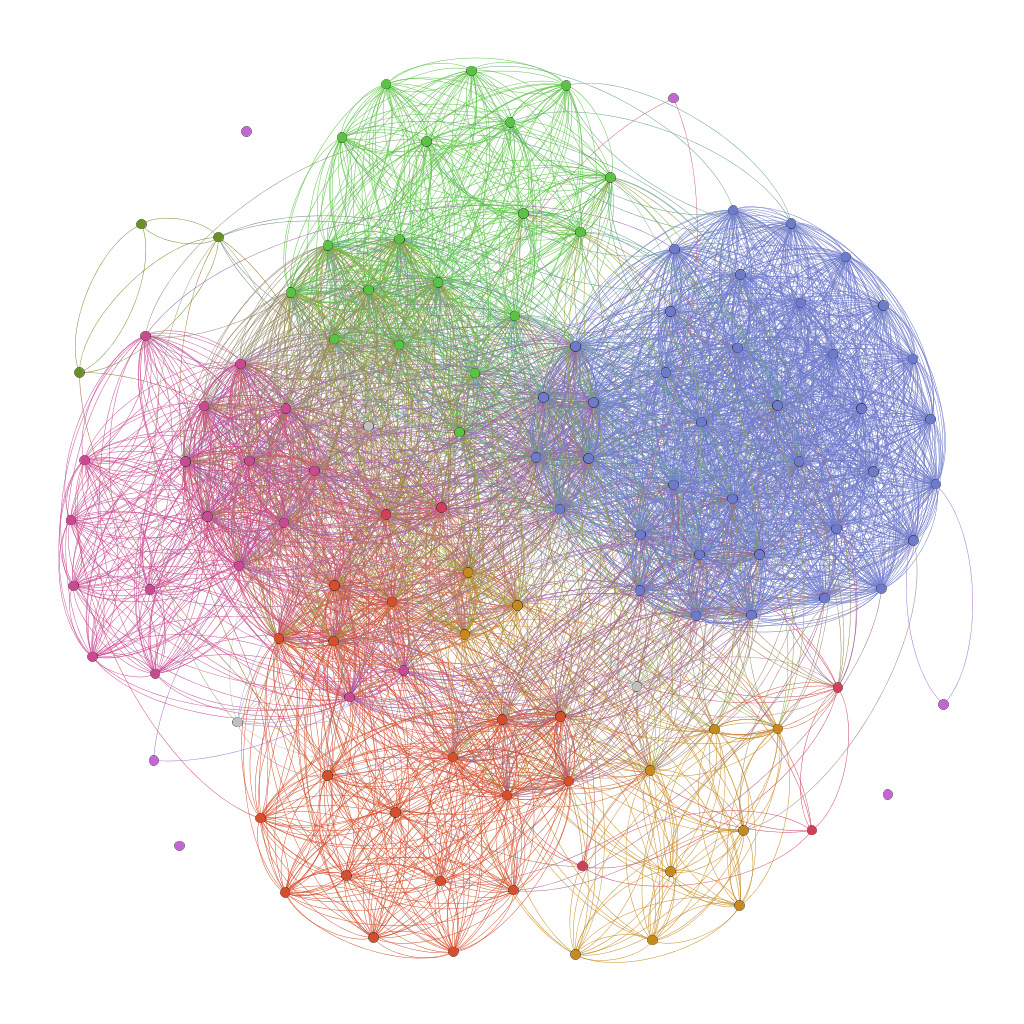
\includegraphics[width=.45\linewidth]{../01.Figures/FR-2010}}
  \subfloat[ForceAtlas2]{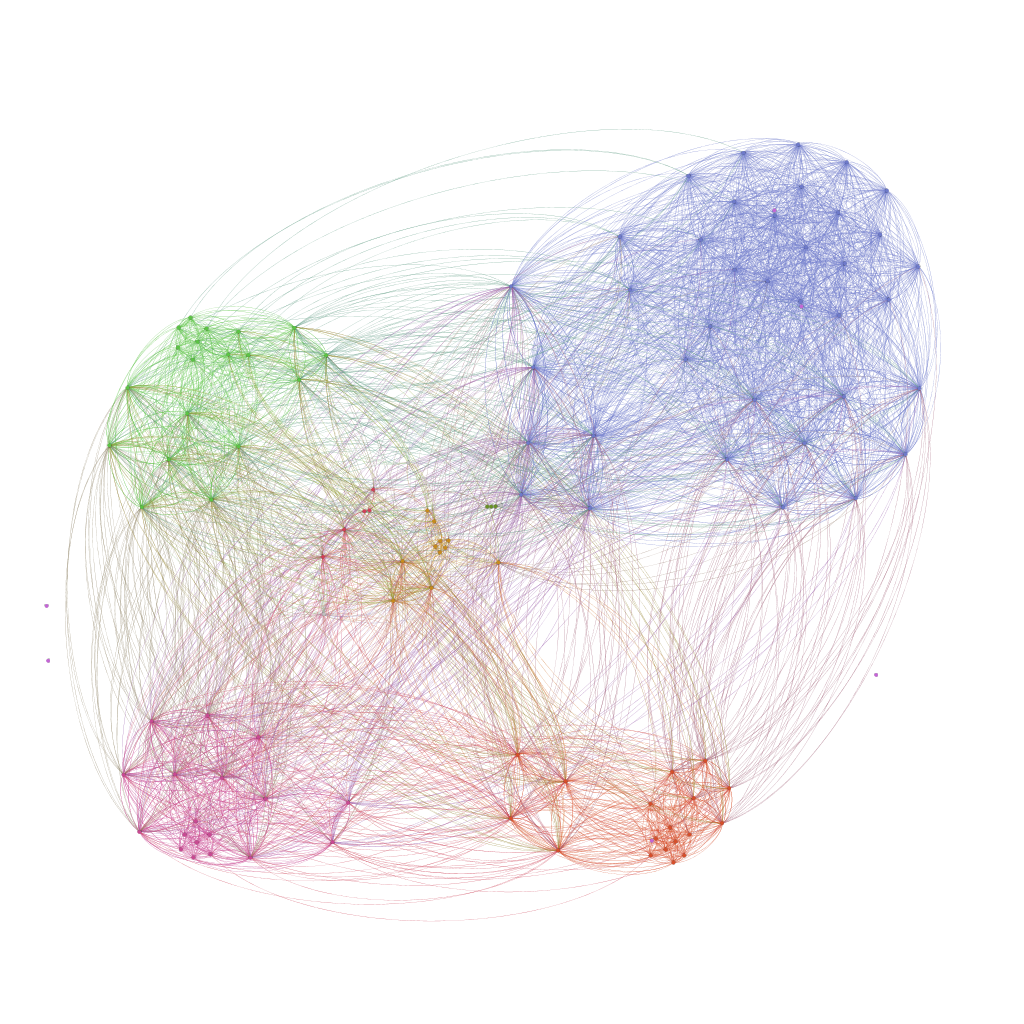
\includegraphics[width=.5\linewidth]{../01.Figures/FA2-2010}}
  \\ \smallskip\noindent\scriptsize Nota: El grafo original con el algoritmo Fruchterman y Reingold fue publicado en escala de grises. En esta versi\'on se utilizan colores para indicar militancia pol\'itica: UDI azul purp\'ureo, PDC malaquita, RN tomate, PPD violeta, PS anaranjado, IND malva, PRSD carmes\'i y PRI verde oscuro.\\
  Fuente: Elaboraci\'on propia con datos de Gonz\'alez-Bustamante y Cisternas (2016).
\end{figure}

\subsection[ForceAtlas2 con algoritmo de modularidad] {ForceAtlas2 con algoritmo de modularidad}

\justify{Indicadores b\'asicos, como la densidad, permiten apreciar que la cantidad de v\'inculos decae desde la segunda legislatura. Al comparar la red m\'as densa (Figura 2), con la de menor densidad (Figura 6), se aprecia una disminuci\'on del 24\% en el indicador. Sin embargo, otras mediciones m\'as sofisticadas, como el algoritmo de modularidad presentado en el apartado metodol\'ogico, permiten evaluar la solidez de las conexiones entre los {\itshape nodos} de un mismo conglomerado o m\'odulo. A mayor modularidad, existen conexiones m\'as s\'olidas dentro del cl\'uster y menor cantidad de v\'inculos con {\itshape alters} de otros m\'odulos.}

\justify{En este sentido, con la aplicaci\'on del algoritmo de modularidad se obtiene que $\Delta Q$(grafo 1) = 0,354; $\Delta Q$(grafo 2) = 0,375; $\Delta Q$(grafo 3) = 0,372; $\Delta Q$(grafo 4) = 0,416; $\Delta Q$(grafo 5) = 0,414; y $\Delta Q$(grafo 6) = 0,409. Con el algoritmo tambi\'en es posible identificar un n\'umero espec\'ifico de comunidades, lo que permite un an\'alisis m\'as detallado de la red. En la primera legislatura se pueden identificar 13 comunidades, en la segunda y tercera ocho, en la cuarta nueve y en las dos \'ultimas legislaturas solo siete comunidades. Esta es una evidencia mucho m\'as precisa que complementa que no solo existen legislaturas menos densas, en t\'erminos de composici\'on social, adem\'as, el n\'umero de cl\'usteres comienza a descender.}

%%%%%%%%%%%%%%%%%%%%%%%%%%%%%%%%%%%%%%%%%%%%%%%%%%

\section[Discusi\'on] {{\normalfont Discusi\'on}}

%%%%%%%%%%%%%%%%%%%%%%%%%%%%%%%%%%%%%%%%%%%%%%%%%%

\justify{En los seis grafos usados para analizar las legislaturas entre 1990 y 1994 en Chile, la aplicaci\'on del algoritmo ForceAtlas2 ofrece una mejor visualizaci\'on y adem\'as permite apreciar de mejor forma los conglomerados que se conforman. Esto ayuda a evitar problemas de interpretaci\'on con respecto a patrones identificables en las redes. Por otra parte, el algoritmo de modularidad permite evaluar con precisi\'on la solidez de las conexiones dentro de los cl\'usteres y delimitar su conformaci\'on a un nivel m\'as desagregado que con una inspecci\'on visual.}

\justify{Esto ayuda a delinear futuras l\'ineas de investigaci\'on que busquen realizar un an\'alisis m\'as espec\'ifico de las conexiones y la conformaci\'on de conglomerados y, de esta forma, evaluar que tan cerrada o abierta es la \'elite de un pa\'is en un momento hist\'orico determinado.}

%%%%%%%%%%%%%%%%%%%%%%%%%%%%%%%%%%%%%%%%%%%%%%%%%%

\section{{\normalfont Referencias}}

%%%%%%%%%%%%%%%%%%%%%%%%%%%%%%%%%%%%%%%%%%%%%%%%%%

\begin{list}{}%
{\leftmargin=1em \itemindent=-1em}

\item{\small Blondel, V. D., Guillaume, J.-L., Lambiotte, R., {\itshape \&} Lefebvre, E. (2008). Fast unfolding of communities in large networks. {\itshape Journal of Statistical Mechanics: Theory and Experiment}, 10, P10008. {\scshape doi:} \href{https://arxiv.org/abs/0803.0476}{\textcolor{blue}{10.1088/1742-5468/2008/10/P10008}}}

\item{\small Bourdieu, P. (1980/2009). {\itshape El sentido práctico}.  Ciudad de México: Siglo XXI Editores.}

\item{\small Brandes, U. (2001). A faster algorithm for betweenness centrality. {\itshape Journal of Mathematical Sociology, 25}(2), 163-177. {\scshape doi:} \href{https://doi.org/10.1080/0022250X.2001.9990249}{\textcolor{blue}{10.1080/0022250X.2001.9990249}}}

\item{\small Bunker, K., {\itshape \&} Navia, P. (2015). Incumbency Advantage and Tenure Length in the Chilean Chamber of Deputies, 1989-2009. {\itshape Revista de Ciencia Pol\'itica, 35}(2), 251-271. {\scshape doi:} \href{http://dx.doi.org/10.4067/S0718-090X2015000200001}{\textcolor{blue}{10.4067/S0718-090X2015000200001}}}

\item{\small Cisternas, C., {\itshape \&} González-Bustamante, B. (2016). {\itshape Los monjes de CIEPLAN: Producción intelectual y redes de citación durante los años ochenta}. Ponencia presentada en el Seminario Internacional “Ciencias sociales en la encrucijada: Intelectuales y tecnócratas latinoamericanos en tiempos de autoritarismo (1969-1990)”, Santiago.}

\item{\small Cisternas, C., {\itshape \&} Vásquez, J. (2018). Comisiones Asesoras Presidenciales en Chile: Entre la expertise y la pluralidad de actores sociales. {\itshape European Review of Latin American and Caribbean Studies}, 106, 1-24. {\scshape doi}: \href{http://doi.org/10.32992/erlacs.10349}{\textcolor{blue}{10.32992/erlacs.10349}}}

\item{\small Cronin, B., {\itshape \&} Shaw, D. (2002). Identity-creators and image-makers: Using citation analysis and thick description to put authors in their place. {\itshape Scientometrics, 54}(1), 31-49. {\scshape doi}: \href{https://doi.org/10.1023/A:1015628320056}{\textcolor{blue}{10.1023/A:1015628320056}}}

\item{\small Eades, P. D. (1984). A heuristic for graph drawing. {\itshape Congressus Nutnerantiunt, 42}, 149-160.}

\item{\small Friedkin, N. E. (1981). The development of structure in random networks: an analysis of the effects of increasing network density on five measures of structure. {\itshape Social Networks, 3}(1), 41-52. {\scshape doi:} \href{https://doi.org/10.1016/0378-8733(81)90004-6}{\textcolor{blue}{10.1016/0378-8733(81)90004-6}}}

\item{\small Fruchterman, T. M. J., {\itshape \&} Reingold, E. M. (1991). Graph drawing by force-directed placement. {\itshape Software: Practice and Experience, 21}(11), 1129-1164. {\scshape doi:} \href{https://doi.org/10.1002/spe.4380211102}{\textcolor{blue}{10.1002/spe.4380211102}}}

%% \item{\small Gonz\'alez-Bustamante, B. (2014). Elecci\'on directa de consejeros regionales 2013. Rendimiento del capital pol\'itico, familiar y econ\'omico en una nueva arena electoral en Chile. {\itshape Pol\'itica, Revista de Ciencia Pol\'itica, 52}(2), 49-91. {\scshape url:} \href{https://revistapolitica.uchile.cl/index.php/RP/article/view/36137}{\textcolor{blue}{https://revistapolitica.uchile.cl}}}

\item{\small Gonz\'alez-Bustamante, B. (2014). Elecci\'on directa de consejeros regionales 2013. Rendimiento del capital pol\'itico, familiar y econ\'omico en una nueva arena electoral en Chile. {\itshape Pol\'itica, Revista de Ciencia Pol\'itica, 52}(2), 49-91.}

\item{\small González-Bustamante, B. (2020). El estudio de las élites políticas gubernamentales en América Latina: Panorama, agendas de investigación y desafíos metodológicos. {\itshape SocArXiv}. {\scshape doi:} \href{https://doi.org/10.31235/osf.io/syqu4}{\textcolor{blue}{10.31235/osf.io/syqu4}}}

%% \item{\small Gonz\'alez-Bustamante, B., {\itshape \&} Cisternas, C. (2016). \'Elites pol\'iticas en el poder legislativo chileno: La C\'amara de Diputados (1990-2014). {\itshape Pol\'itica, Revista de Ciencia Pol\'itica, 54}(1), 19-52. {\scshape url:} \href{https://revistapolitica.uchile.cl/index.php/RP/article/view/42691}{\textcolor{blue}{https://revistapolitica.uchile.cl}}}

\item{\small Gonz\'alez-Bustamante, B., {\itshape \&} Cisternas, C. (2016). \'Elites pol\'iticas en el poder legislativo chileno: La C\'amara de Diputados (1990-2014). {\itshape Pol\'itica, Revista de Ciencia Pol\'itica, 54}(1), 19-52.}

\item{\small Gonz\'alez-Bustamante, B., {\itshape \&} Olivares, A. (2015). Rotaci\'on de subsecretarios en Chile: Una exploraci\'on de la segunda l\'inea gubernamental, 1990-2014. {\itshape Revista de Gesti\'on P\'ublica, IV}(2), 151-190. {\scshape doi:} \href{https://doi.org/10.22370/rgp.2015.4.2.2230}{\textcolor{blue}{10.22370/rgp.2015.4.2.2230}}}

%% \item{\small Gonz\'alez-Bustamante, B., {\itshape \&} Olivares, A. (2018). La \'elite pol\'itica gubernamental en Chile: Supervivencia de ministros (1990-2014). En A. Codato {\itshape \&} F. Espinoza (eds.),{ \itshape Las \'Elites en las Am\'ericas: Diferentes Perspectivas}. Curitiba: Editora Universidade Federal do Paran\'a. \\ {\scshape url:} \href{https://www.researchgate.net/publication/325699783_Elites_en_las_Americas_diferentes_perspectivas_Elites_in_the_Americas_Different_Perspectives}{\textcolor{blue}{https://www.researchgate.net}}}

\item{\small Gonz\'alez-Bustamante, B., {\itshape \&} Olivares, A. (2018). La \'elite pol\'itica gubernamental en Chile: Supervivencia de ministros (1990-2014). En A. Codato {\itshape \&} F. Espinoza (eds.),{ \itshape Las \'Elites en las Am\'ericas: Diferentes Perspectivas}. Curitiba: Editora Universidade Federal do Paran\'a.}

\item{\small Hanneman, R. A., {\itshape \&} Riddle, M. (2005). {\itshape Introduction to Social Networks Methods}. Riverside: University of California Riverside.}

\item{\small Jacomy, M., Venturini, T., Heymann, S., {\itshape \&} Bastian, M. (2014). ForceAtlas2, a Continuous Graph Layout Algorithm for Handy Network Visualization Designed for the Gephi Software. {\itshape PLoS ONE, 9}(6), e98679. {\scshape doi:} \href{https://doi.org/10.1371/journal.pone.0098679}{\textcolor{blue}{10.1371/journal.pone.0098679}}}

%% \item{\small Joignant, A. (2014). El capital pol\'itico familiar: Ventajas de parentela y concentraciones de mercado en las elecciones generales chilenas 2013. {\itshape Pol\'itica, Revista de Ciencia Pol\'itica, 52}(2), 13-48. {\scshape url:} \href{https://revistapolitica.uchile.cl/index.php/RP/article/view/36134}{\textcolor{blue}{https://revistapolitica.uchile.cl}}}

\item{\small Joignant, A. (2014). El capital pol\'itico familiar: Ventajas de parentela y concentraciones de mercado en las elecciones generales chilenas 2013. {\itshape Pol\'itica, Revista de Ciencia Pol\'itica, 52}(2), 13-48.}

\item{\small Maillet, A., Gonz\'alez-Bustamante, B., {\itshape \&} Olivares, A. (2016). ?`Puerta giratoria? An\'alisis de la circulaci\'on p\'ublico-privada en Chile (2000-2014). {\itshape Serie de Documentos de Trabajo PNUD-Desigualdad}, 7,  1-40. \\ {\scshape doi:} \href{https://doi.org/10.13140/RG.2.2.25510.42566}{\textcolor{blue}{10.13140/RG.2.2.25510.42566}}}

\item {\small Newman, M. E. J., {\itshape \&} Girvan, M. (2004). Finding and evaluating community structure in networks. {\itshape Physical Review E, 69}(2), 026113-1-026113-15. {\scshape doi:} \href{https://doi.org/10.1103/PhysRevE.69.026113}{\textcolor{blue}{10.1103/PhysRevE.69.026113}}}

\item{\small Noack, A. (2007a). Energy Models for Graph Clustering. {\itshape Journal of Graph Algorithms and Applications, 11}(2), 453-480. {\scshape doi:} \href{http://dx.doi.org/10.7155/jgaa.00154}{\textcolor{blue}{10.7155/jgaa.00154}}}

\item{\small Noack, A. (2007b). {\itshape Unified Quality Measures for Clusterings, Layouts, and Orderings of Graphs, and Their Application as Software Design Criteria}. (Ph. D. Tesis), Brandenburg University of Technology Cottbus-Senftenberg.}

\item{\small Noack, A. (2009). Modularity clustering is force-directed layout. {\itshape Physical Review E, 79}(2), 026102-2-026102-8. {\scshape doi:} \href{https://doi.org/10.1103/PhysRevE.79.026102}{\textcolor{blue}{10.1103/PhysRevE.79.026102}}}

\item{\small Olivares, A., González-Bustamante, B., Toro Maureira, S., Arellano, J. C., Yanes-Rojas, A., Zurita-Tapia, J., Lopes, A. V., Robledo Guzmán, C., {\itshape \&} Canavesi Sosa, J. B. (2020). Nuevos desafíos, enfoques y perspectivas para estudiar élites políticas. {\itshape Iberoamericana, XX}(74), 229-259. \\ {\scshape doi:} \href{http://doi.org/10.18441/ibam.20.2020.74.229-259}{\textcolor{blue}{10.18441/ibam.20.2020.74.229-259}}}

%% \item{\small Salda\~na, J. (2014). Carreras pol\'iticas de los diputados chilenos, 1989-2013: evoluci\'on y sus consecuencias para la representaci\'on pol\'itica del pa\'is. {\itshape Pol\'itica, Revista de Ciencia Pol\'itica, 52}(2), 127-155. \\ {\scshape url:} \href{https://revistapolitica.uchile.cl/index.php/RP/article/view/36139}{\textcolor{blue}{https://revistapolitica.uchile.cl}}}

\item{\small Salda\~na, J. (2014). Carreras pol\'iticas de los diputados chilenos, 1989-2013: evoluci\'on y sus consecuencias para la representaci\'on pol\'itica del pa\'is. {\itshape Pol\'itica, Revista de Ciencia Pol\'itica, 52}(2), 127-155.}

\item{\small Wasserman, S., {\itshape \&} Faust, K. (1994). {\itshape Social Network Analysis: Methods and Applications}. Nueva York: Cambridge University Press.}

\item{\small White, H. D. (2001). Authors as citers over time. {\itshape Journal of the American Society for Information Science and Technology, 52}(2), 87-108. {\scshape doi}: \href{https://doi.org/10.1002/1097-4571(2000)9999:9999\%3C::AID-ASI1542\%3E3.0.CO;2-T}{\textcolor{blue}{10.1002/1097-4571(2000)}}}
\end{list}

%%%%%%%%%%%%%%%%%%%%%%%%%%%%%%%%%%%%%%%%%%%%%%%%%%

\vspace{8mm}
\section[Informe de revisión]{\LARGE \itshape Informe abierto de revisi\'on}

%%%%%%%%%%%%%%%%%%%%%%%%%%%%%%%%%%%%%%%%%%%%%%%%%%

\vspace{8mm}
{\noindent {\Large Alejandro Olivares L.} \footnote{Profesor Asociado, Departamento de Sociología y Ciencia Política, Facultad de Ciencias Sociales y
Humanidades, Universidad Católica de Temuco. ORCID iD: \href{https://orcid.org/0000-0001-6934-2437}{\textcolor{blue}{0000-0001-6934-2437}}} \\
{\normalsize Universidad Católica de Temuco} \\
\vspace{1mm}{\LARGE \Letter} \href{mailto:alejandro.olivares@uct.cl}{\textcolor{blue}{\normalsize alejandro.olivares@uct.cl}}}
\vspace{8mm}

\justify{Se trata de un documento de trabajo que constituye un aporte al campo de estudio de las élites, particularmente entre aquellos investigadores que buscan analizar las conexiones (redes) que existen dentro de las élites políticas, económicas y sociales. Se propone una mejora a la forma en que se presentan los conglomerados de las redes analizadas.  El uso grafos para identificar grupos o comunidades permite visualizar la forma en que se agrupan las conexiones y el alcance de las redes. No obstante, al momento de publicar los hallazgos se pueden generar problemas visuales que dificultan, para un lector menos especializado, la interpretación de los resultados, toda vez que la presentación de los grafos no es amigable, los puntos se solapan y puede ser difícil en un artículo analizar los efectos.  Esto, tal como proponen los autores se soluciona con el algoritmo ForceAtlas2 que permite “una mejor visualización y además permite apreciar de mejor forma los conglomerados que se conforman”. Esto se logra muy bien en el trabajo.}

\justify{Uno de los aspectos que el documento podría mejorar es la forma en que se presenta el texto. La entrada es muy directa y falta contextualización sobre la importancia del estudio de redes y la lógica de los grafos y del análisis de redes. En ese sentido se recomienda dedicar al menos un párrafo para orientar al lector sobre la importancia de estas lógicas.  Del mismo modo, es relevante señalar en la introducción de forma más clara el objetivo del trabajo. Sería suficiente con dos líneas que indiquen que se busca demostrar que introduciendo mejoras como el algoritmo ForceAtlas2 es posible realizar un análisis más específico de las conexiones y la conformación de conglomerados y, de esta forma, evaluar que tan cerrada o abierta es la élite analizada.}

\justify{Por otra parte, la discusión final podría extenderse un poco más. Para un trabajo tan bien desarrollado el cierre podría profundizar un poco más en, por ejemplo, las limitaciones potenciales del algoritmo o bien destacar más sus potenciales no solo para el análisis de las élites políticas, sino que para redes en general y élites de todo tipo. A pesar de estas potencialidades es relevante tener en cuenta que esto ofrece ventajas analíticas más bien descriptivas que debiesen complementarse con modelos estocásticos para redes dinámicas con el objetivo de analizar cambios de patrones y estimar parámetros que afectan las probabilidades de establecer relaciones.}

%%%%%%%%%%%%%%%%%%%%%%%%%%%%%%%%%%%%%%%%%%%%%%%%%%

\section{{\normalfont CRediT -- Contributor Roles Taxonomy}}

%%%%%%%%%%%%%%%%%%%%%%%%%%%%%%%%%%%%%%%%%%%%%%%%%%

{\noindent {\bfseries Bastián González-Bustamante} (autor/editor)}

{\noindent {\includegraphics[width=.085\linewidth]{../../badges/conceptualization} {\includegraphics[width=.085\linewidth]{../../badges/data_curation} {\includegraphics[width=.085\linewidth]{../../badges/formal_analysis} {\includegraphics[width=.085\linewidth]{../../badges/funding_acquisition} {\includegraphics[width=.085\linewidth]{../../badges/methodology} {\includegraphics[width=.085\linewidth]{../../badges/project_administration} {\includegraphics[width=.085\linewidth]{../../badges/computation} {\includegraphics[width=.085\linewidth]{../../badges/data_visualization} {\includegraphics[width=.085\linewidth]{../../badges/writing_initial_draft}
{\includegraphics[width=.085\linewidth]{../../badges/writing_review}}\\

{\noindent {\bfseries Carla Cisternas} (autora)}

{\noindent {\includegraphics[width=.085\linewidth]{../../badges/conceptualization}
{\includegraphics[width=.085\linewidth]{../../badges/data_curation} {\includegraphics[width=.085\linewidth]{../../badges/formal_analysis}
{\includegraphics[width=.085\linewidth]{../../badges/investigation} {\includegraphics[width=.085\linewidth]{../../badges/computation} {\includegraphics[width=.085\linewidth]{../../badges/testing} {\includegraphics[width=.085\linewidth]{../../badges/data_visualization} {\includegraphics[width=.085\linewidth]{../../badges/writing_initial_draft}
{\includegraphics[width=.085\linewidth]{../../badges/writing_review}}\\

{\noindent {\bfseries Jaquelin Morillo} (editora)}

{\noindent {\includegraphics[width=.085\linewidth]{../../badges/writing_review}}\\

{\noindent {\bfseries Alejandro Olivares L.} (evaluador)}

{\noindent {\includegraphics[width=.085\linewidth]{../../badges/writing_review}}\\

{\noindent {\bfseries Elinor Luco} (asistente editorial)}

{\noindent {\includegraphics[width=.085\linewidth]{../../badges/writing_review}}

%%%%%%%%%%%%%%%%%%%%%%%%%%%%%%%%%%%%%%%%%%%%%%%%%%

\section{{\normalfont Historial de revisiones}}

%%%%%%%%%%%%%%%%%%%%%%%%%%%%%%%%%%%%%%%%%%%%%%%%%%

\vspace{-0.6cm}
\begin{table}[h]
\begin{tabular}{@{}lll@{}}
{\small 1,0} & {\small 13 noviembre 2018} & {\small Manuscrito original} \\[0.8mm]
{\small 2,0} & {\small 10 agosto 2020} & {\small Manuscrito revisado} \\[0.8mm]
{\small 3,0} & {\small 13 septiembre 2020} & {\small Fecha de publicación} \\[0.8mm]
{\small 4,0} & {\small 20 abril 2021} & {\small Correcciones menores}\\[0.8mm]
{\small 5,0} & {\small 30 diciembre 2021} & {\small Correcciones menores} \\[0.8mm]
{\small 6,0} & {\small 7 abril 2022} & {\small Correcciones menores} \\[0.8mm]
{\small 7,0} & {\small 25 abril 2022} & {\small Correcciones menores} \\
\end{tabular}
\end{table}
\vspace{0.3cm}
{\noindent \footnotesize {\normalsize \faCloudDownload} Descargar la versión más reciente desde SocArXiv ({\scriptsize DOI:} \href{https://doi.org/10.31235/osf.io/gxrkc}{\textcolor{blue}{10.31235/osf.io/gxrkc}}).}

\end{document}
